\documentclass[12pt,letterpaper,twoside]{article}
\usepackage[english]{babel}

%% Layout and Style
\usepackage{fancyhdr}
\frenchspacing          % Spacing between sentences
\usepackage{paralist,booktabs}  % compactlist, compactitem, and nice tables
\usepackage{tocloft}   % Spacing in Table of Contents
\renewcommand{\cftbeforesecskip}{1.5pt}

%% Math
\usepackage{amssymb,amsmath,amsthm} % Standard Math symbols, operators, and environments
\usepackage[nice]{nicefrac}  % Better small fractions
\usepackage{esint,cases}     % \oiint, \iint, and function case construction

%% Graphics
\usepackage{graphicx}
\usepackage{pgf,pgffor,pgfplots,pgfplotstable}
\usepgfmodule{shapes,plot}
\usepackage{tikz}
\usetikzlibrary{decorations,arrows,decorations}
%\graphicspath{{./images/}}   % Where to find images

%% Hyperlink sections, references, and citations
\definecolor{LinkBlue}{RGB}{5,10,200}
\usepackage[urlcolor=LinkBlue,linkcolor=LinkBlue,citecolor=LinkBlue,colorlinks=true]{hyperref}
\usepackage{url}

%% Problems and Questions
\newcommand{\problem}[1]{\newpage\addtocounter{section}{1}\phantomsection\addcontentsline{toc}{section}{#1}\section*{#1}}
\newcommand{\subproblem}[1]{\phantomsection\addcontentsline{toc}{subsection}{#1}\subsection*{#1}}
\newcommand{\subsubproblem}[1]{\phantomsection\addcontentsline{toc}{subsubsection}{#1}\subsubsection*{#1}}

\newcommand{\FatFactor}{0.99}

%% Margins
\oddsidemargin  0in \evensidemargin 0in \topmargin -0.5in
\headheight 0.25in \headsep 0.25in
\textwidth   6.5in \textheight 9in %\marginparsep 0pt \marginparwidth 0pt
\parskip 1.5ex  \parindent 0ex \footskip 20pt

%% Header
\newcommand*{\MyNumberOfPages}{\hypersetup{linkcolor=black}\pageref{NumberOfPages}\hypersetup{linkcolor=blue}}
\newfont{\bssnine}{cmssbx10 scaled 900}
\pagestyle{fancy}
\fancyhead{\bssnine ComputeFest 2013 Computational Challenge}
\fancyhead[RE]{} 
\fancyhead[LO]{}
\fancyhead[LE]{\bssnine \arabic{page}/\MyNumberOfPages} 
\fancyhead[RO]{\bssnine \arabic{page}/\MyNumberOfPages}
\lfoot{} \cfoot{} \rfoot{}

\begin{document}

%% First page header:
\thispagestyle{empty}\vspace*{-0.75in}
\newfont{\bssten}{cmssbx10}
\begin{minipage}[t]{0.5\linewidth}
  {\bssten Institute for Applied Computational Science \\
           ComputeFest 2013 \\
           Computational Challenge Competition}
\end{minipage}
\begin{minipage}[t]{0.5\linewidth}
  \vspace*{-22pt} \raggedleft 
\includegraphics[scale=0.5]{SEAS_IACS}
\end{minipage}

\vspace*{12pt}
{\centering \textbf{ComputeFest 2013 Computational Challenge}{ \par}}
\vspace*{-8pt}\noindent\rule{\linewidth}{1pt}

ComputeFest is an annual extravaganza of skill- and knowledge-building activities for students and researchers interested in computational science and engineering, organized by the Institute for Applied Computational Science at SEAS.

In January 2012, IACS organized the first Computational Challenge. Two student teams competed on an optimization problem: how to get medical aid to the maximum number of victims stranded by a hurricane striking the city of Cambridge. The arrival of superstorm Sandy in October 2012 showed that such a problem definition is hardly far-fetched. 

Chris Beaumont of the Harvard-Smithsonian Center for Astrophysics and Blessing Okeke of SEAS were the team whose approach saved the most hypothetical victims, winning them a pair of iPads.

This year, in place of a single problem judged at the end of a computing run, we invite students to participate in a game. This year's challenge will be a little more light-hearted, but equally challenging: a computational foosball game. Here are the rules of the game. May the best team win!
%
\vspace{4em}
\def\contentsname{\empty}
\tableofcontents

\problem{2013 World Cup comFoosball Competition}
\begin{center}
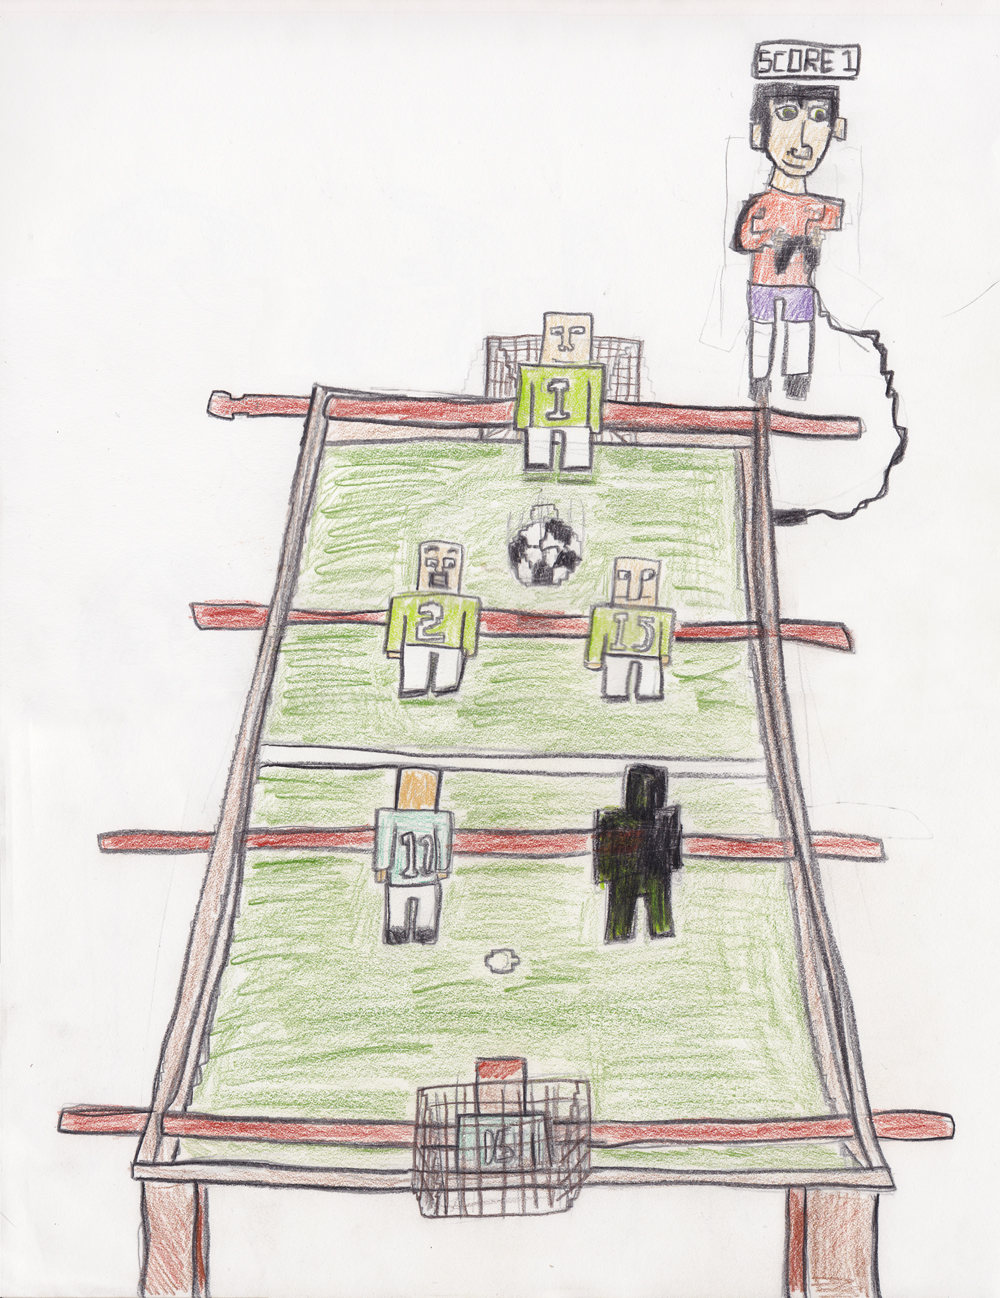
\includegraphics[width=3in]{Foosball_5s}
\end{center}

Foosball is a table-top game invented in 1923. Two teams, from opposite sides of the table, operate plastic figures (``foosplayers"), which are attached to rotating and sliding axles, in order to kick the ball into the opponent's goal. After a point is scored, play is resumed from mid-field. Foosplayers are also used to block and pass the ball. In this computational challenge, we define a simple game modeled after soccer and foosball. 

Your goal is to provide an AI that can play our version of foosball/soccer by strategically optimizing player positions. Your computational strategy for determining the rosters of your foosplayers (deemed your ``foosteam") will be pitted against other foosteams in the foosplayoff tournament.

In the following sections, we define the game that you will be playing in this competition. There are many possible approaches to the problem that speak to the core of computational science: stochastic analysis, optimization, software design, high performance computing, etc. We hope that you use your talents to crush your opposition.

\newpage

\subproblem{Definitions}

\begin{figure}[h!]
\begin{center}
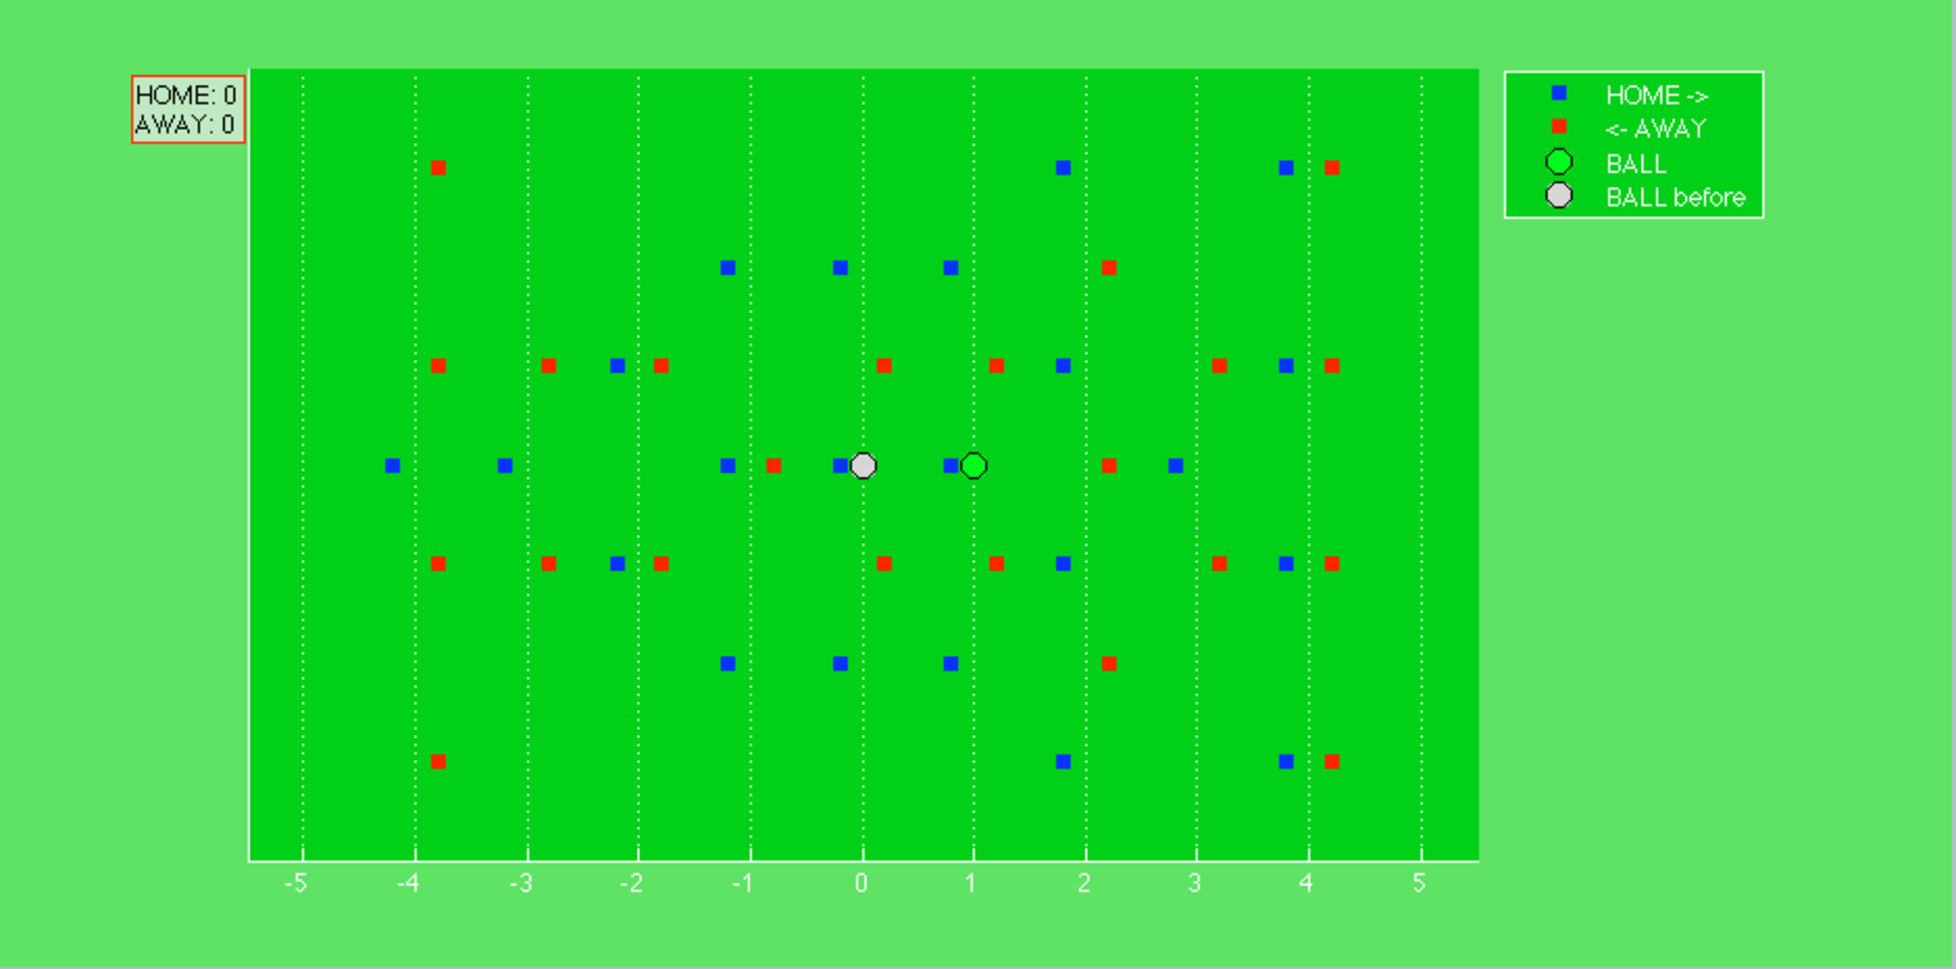
\includegraphics[width=.8\textwidth]{Setup0.pdf} 
\caption{\label{fig:setup} A typical starting line-up. Blue players are the {\em HOME} team and red players are the {\em AWAY} team. {\em HOME} team moves the ball to the right and {\em AWAY} team moves the ball to the left. The current ball position is shown as a green circle. Also shown is the previous ball position shown as light gray circle.}
\end{center}
\end{figure}

\underline{Field:} The field consists of nine rows: -4, -3, -2, -1, 0, 1, 2, 3, and 4. The positive rows are the offensive side, the negative rows are the defensive side, and zero is the {\em midfield}. Rows -5 and 5 are the ``goals" of the board.

\underline{Teams:} The game is played with two teams, the {\em HOME} team and the {\em AWAY} team. Each team is composed of 26 foosplayers. At any given moment, 22 foosplayers from each team must be on the field.

\underline{Foosplayer:} Each fielded foosplayer is placed in a row. Foosplayers of the {\em HOME} team always try to kick the ball to the right (towards row 5), while foosplayers of the {\em AWAY} team always try to kick the ball left (towards row -5). Foosplayer $i$ also has a fatigue level $e_i$. The fatigue increases as the play goes on (see Section {\em Gameplay} below for details).

\underline{Ball:} The ball begins in the mid-field and is advanced once per round in a direction determined by the foosplayers on the ball's current row (see Section {\em Gameplay}). If the ball reaches row 5, the {\em HOME} team scores a point. If the ball reaches row -5, the {\em AWAY} team scores a point. When a point is scored, the ball is reset to midfield. 


\newpage 
\subproblem{Gameplay}

At the start of each game, each team submits its initial roster to distribute the foosplayers to the rows. Each foosplayer $i$ has initial fatigue $e_i = 0$.

Play begins by placing the {\em ball} at mid-field (row zero). Then,
\begin{enumerate}
\item Let the ball be in row $B$. All foosplayers on row $B$ compete to determine the direction the ball is moved: Let $\mathcal{H}$ and $\mathcal{A}$ be the set of foosplayers from the {\em HOME} and {\em AWAY} teams on row $B$ and let $\mathcal{F} = \mathcal{H}\cup \mathcal{A}$. Let $r \in [0,1)$ be a uniform random number. Then,
\begin{align*}
\text{If } r
\begin{Bmatrix}
< \\
> \\
=
\end{Bmatrix}
\frac{\sum_{i\in\mathcal{H}} \FatFactor^{e_i}}{\sum_{i\in\mathcal{F}} \FatFactor^{e_i}} 
\text{ then the ball is }
\begin{cases}
\text{moved to row $B+1$} \\
\text{moved to row $B-1$} \\
\text{kept at row $B$}
\end{cases}
\end{align*}
That is, the fatigue $e_i$ of the foosplayers on row $B$ determine the probability that the {\em HOME} team (and the {\em AWAY} team) advances the ball.

In the case that row $B$ contains no foosplayers ($\mathcal{F} = \emptyset$) then the ball is advanced to row $B+1$ or $B-1$ with probability $0.5$.

%Matched players compete, where each player's chance of winning, and transitioning play toward the opponent's goal, is a function of the number of players and endurance compared to his opponent's. Random draws are done to determine who wins. Let the $r$ be a random number drawn from a uniform distribution between $0 \ldots 1$.
%\begin{eqnarray}
%\rm{IF: \,\,\,\,} && r > \frac{\sum_i e_i^H}{ \sum_i e_i^A+\sum_i e_i^H} \;\; \; \Rightarrow  \rm {MOVE\,\,\,RIGHT} \nonumber \\
%\rm{IF: \,\,\,\,} &&r < \frac{\sum_i e_i^H}{ \sum_i e_i^A+\sum_i e_i^H}  \;\; \;   \Rightarrow  \rm {MOVE\,\,\,LEFT}  \nonumber  \\
%\rm{IF: \,\,\,\,} && r = \frac{\sum_i e_i^H}{ \sum_i e_i^A+\sum_i e_i^H}   \;\; \;  \Rightarrow  \rm {STAY} \nonumber \\
%\end{eqnarray}
%When a player wins, ball moves to her right, in the direction of the opposing team's goal. A goal is scored when the ball reaches the end of the field. Game play resumes from mid-field.

\item If the new ball position is a goal row, the appropriate team earns a goal and the ball is reset to midfield.

\item Once the new ball position is determined, every foosplayer in row $B$ that competed to advance the ball is hit with fatigue:
\begin{align*}
\text{For all } i \in \mathcal{F}, \ \ e_i \leftarrow e_i + 1
\end{align*}

\item After the ball is advanced and the players fatigued, each team may move any one foosplayer from its current row to an adjacent row.

\item Repeat for 200 rounds.

\item Every 200 rounds, a new quarter begins. To begin a new quarter, each team may submit am entirely new roster. That is, foosplayers may be placed in any row. Note that all fooplayers that were ``benched" in the previous quarter have no fatigue ($e_i = 0$).

\item Repeat for 4 quarters.

\item The team with the most goals wins the game.
\end{enumerate}




%\subproblem{Players}
%\label{sec:Players}
%Player $i$ starts with initial endurance $e_i (t=0)=1$. 
% 
%Each player suffers exhaustion to his endurance every time he/she competes in a random draw. Exhaustion dynamics follow a population ``fatigue curve" modeled as 
%\[ e_i(t) = \FatFactor \,  e_i(t-1).\]
%
%Every player that participates in a draw suffers  fatigue independently of the number of players in
%the \PR. For example, say the ball is at \PR-1, and team-HOME has three players and team-AWAY has one player in that raw, 
%after a draw all four players' endurance would be reduced by a factor of \FatFactor.
%
%Players totally recover when are not on the field (are substituted). 
% 
% Figure \ref{fig:setup2} shows the state of the game after 200 time steps. The endurance of players is indicated 
%with the color intensity. Players in the middle rows tend to fatigue faster because the ball tends to 
%stay in the middle the longest. This should be part of the strategy facing an opponent. 
%%Enhanced Version: Each player also has a ``learning curve" which improves his skill level linearly with each win. Players differ in only initial endowments of skill level and endurance, corresponding to different player types. Initial endowments are drawn from distributions and are the same for each team. 
% 
% 
%\begin{figure}[h!]
%\begin{center}
%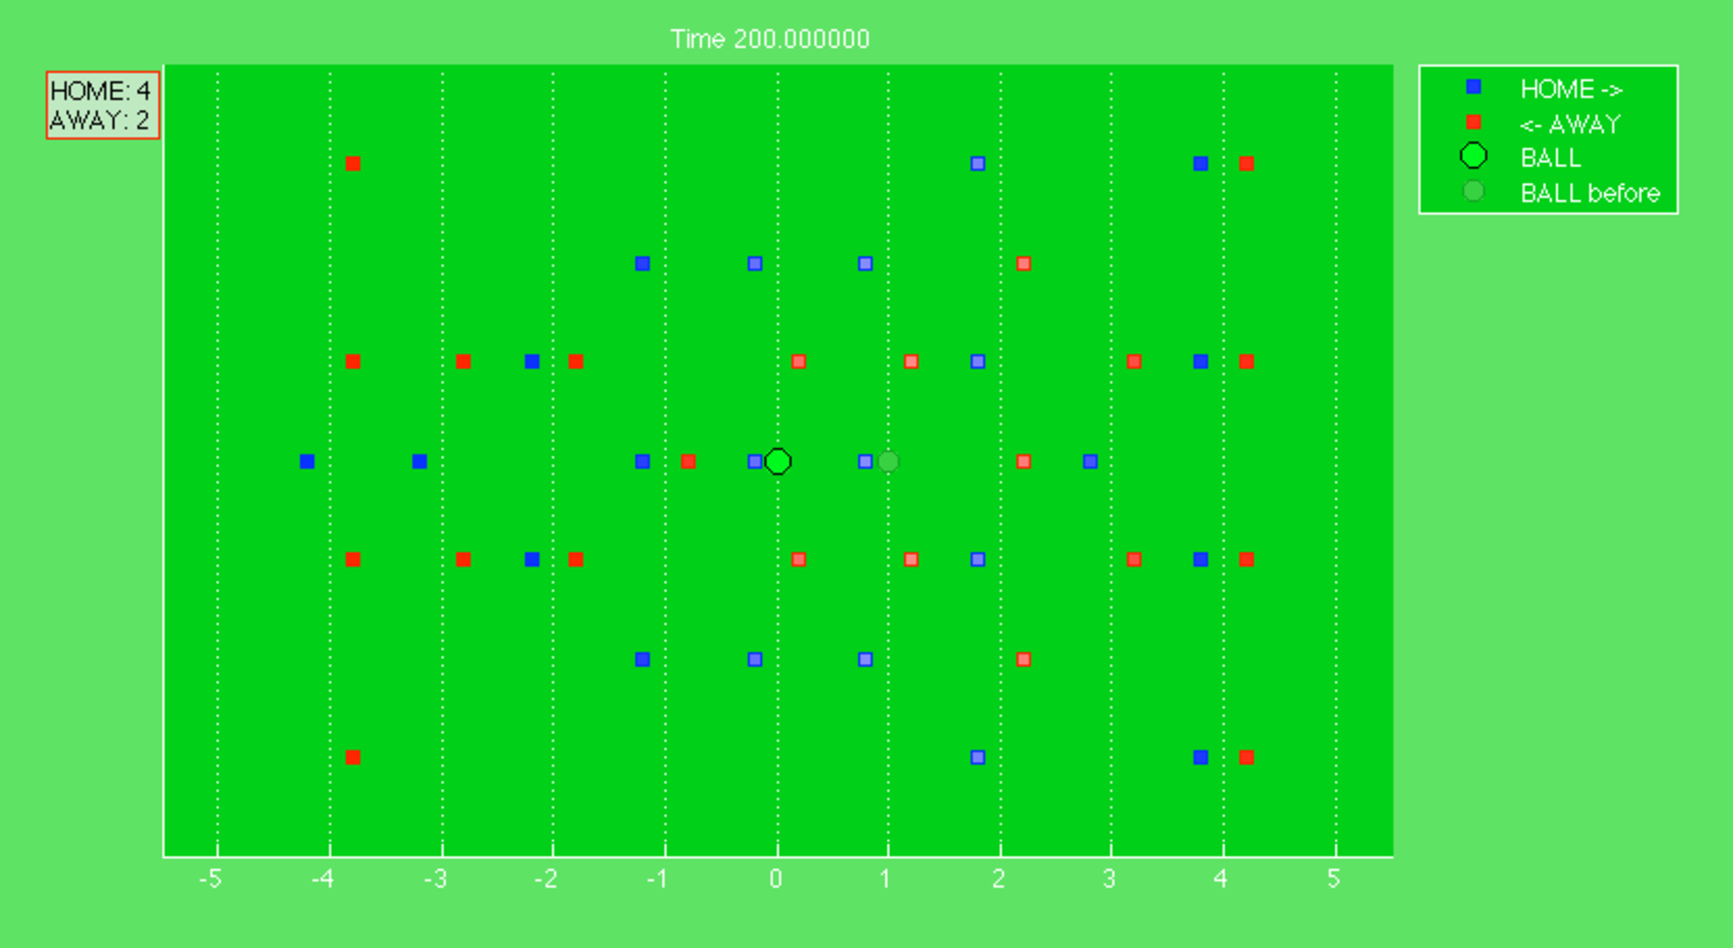
\includegraphics[width=.8\textwidth]{Setup.pdf} 
%\caption{\label{fig:setup2} A state of the game after 200 time steps. The endurance of players is indicated 
%with the color intensity. Players in the middle rows tend to fatigue faster because the ball tends to 
%stay in the middle the longest. }
%\end{center}
%\end{figure}

\newpage 
\subproblem{Roster}

A roster is an array that maps foosplayer number to foosplayer row position. Each foosteam has 26 foosplayers with exactly 22 foosplayers on the field during any round. The $i$th value is the $i$th foosplayers' row position. For example:
\begin{verbatim}
-4 -4 3 3 100 4 -3 -3 -2 -2 -2 -1 -1 -1 0 2 2 0 1 1 1 1 100 100 4 100
\end{verbatim}
Row positions that are outside the range $[-4,4]$ are considered ``benched" and not in play. Negative row numbers are always defensive positions and positive row numbers are always offensive positions.

Foosteams submit the entire roster each round. If an invalid roster is submitted, the game will print a warning, reject the play, and accept the null move -- no change to foosplayers' positions will be made.

Most rounds, the roster can only change by a single foosplayer's row position to an adjacent row. However, when the round number is 0, 200, 400, and 600, a new quarter is about to begin and any valid roster will be accepted.

%\subproblem{Substitutions}
%
%After $\NTR$ moves,  teams are allowed to make up to \NumSubstitutions~substitutions.
%At the end of a \SEC, the referee calls for substitutions. Teams have \SubTime~minutes to upload (see below on details on how
%to upload and what format) the next rotation.
%After the substitutions are completed, play starts at the same place where the game was stopped. 
%
%Substitution is when a player from the bench is inserted into the game. 
%Position change of a player that is already in the field is not considered a
%substitution. There are no limit on the number of position changes.
%
%
%\subproblem{Extra Time}
%In the event that a game is finished in a tie during the elimination phase (see {\em League} below for a description), there will be two extra \SEC s. 
%If the game is still a tie after those two periods, there will be a sudden death session. 
%First team that scores is the winner. 
%
%\subproblem{Winner}
%Winner is the team with the highest number of goals.

\subproblem{Game State}

When both foosteams have submitted their rosters (valid or invalid) the game will continue to the next round by updating the foosplayer positions, the foosplayer fatigues, the ball position, the foosteam scores, and the round number. These are communicated back to the foosteam as a single array ({\bf Note: $0$-indexed}):

\begin{verbatim}
game_state[0]: team score
game_state[1]: opponent team score
game_state[2]: game round number
game_state[3]: row number of the ball
game_state[ 4]-[ 29]: team foosplayer row positions
game_state[30]-[ 55]: team foosplayer fatigues
game_state[56]-[ 81]: opponent foosplayer row positions
game_state[81]-[107]: opponent foosplayer fatigues
\end{verbatim}

This game state should then be used to choose a roster for the next round.

\newpage
\subproblem{Game Engine}

We will be using a centralized game engine that keeps track of the game state and allows any programming language to communicate with it. This makes it easy to pit foosteams of different types and languages against each other.

You may download a selection of skeleton code that has been written to get you started communicating with this game engine:
\begin{center}
\href{http://crisco.seas.harvard.edu/ComputeFest2013/Codes.zip}{\large\bf Download codes here}\\
or \\
{\tt wget http://crisco.seas.harvard.edu/ComputeFest2013/Codes.zip}
\end{center}
These codes provide communication clients and skeleton foosteams in Python, Matlab, C++, and Java.

To play two foosteams against each other, launch both foosteams with the same commandline game ID. For example:
\begin{verbatim}
$ python foosteam.py 1234
Waiting for game 1234
\end{verbatim}
launches a foosteam into a game with ID 1234. Another foosteam can join this game by launching with the same game ID:
\begin{verbatim}
# After compiling with 'javac *.java'
$ java foosteam 1234
Waiting for game 1234
READY
\end{verbatim}
The second foosteam is in Java here, but could also be the same Python foosteam from above.

Once two foosteams have joined a game, {\tt READY} is broadcast to both foosteams and the game loop is entered. Both teams submit their first roster, receive the game state, decide on their next roster, etc, until the game is over.





You will be editing the {\tt foosteam} file in the language of your choice: specifically, the {\tt new\_move} function, which takes a game state and returns a roster for that game round.


\newpage
\subproblem{Competition}
\subsubproblem{Time/Location}
The final competition will be held on Wednesday at 1:30pm at MD119.

\subsubproblem{Roud-robin phase}
There are 10 teams. 

Each team will face all other teams in 45 {\em matches} (see Table \ref{tab:rr}).
A match is composed of 5 games. 
 
The team that wins the most games in a match is awarded 2 points.
If the two teams win the same number of games, 1 point is awarded
to each team. The losing team is awarded zero points. 

\begin{table}[htdp]
\caption{\label{tab:rr}The round-robin competition}
\begin{center}
\begin{tabular}{|c|ccccc|}
\hline
Round 1 &     1-10 &   2-9  &  3-8 &   4-7 &   5-6   \\
Round 2 &    1-9 &  2-7   & 3-6    &  4-5  &  8-10   \\
Round 3 &     1-8 & 2-5   & 3-4   & 6-10 &  7-9  \\
Round 4 &     1-7 & 2-3   & 4-10   & 5-9 &  6-8  \\
Round 5 &     1-6 & 2-10   & 3-9   & 4-8 &  5-7  \\
Round 6 &     1-5 & 2-8   & 3-7   & 4-6 & 9-10  \\
Round 7 &     1-4 & 2-6   & 3-5   & 7-10 &  8-9  \\
Round 8 &     1-3 & 2-4   & 5-10   & 6-9 &  7-8 \\
Round 9 &     1-2 & 3-10   &  4-9   & 5-8 & 6-7    \\
\hline
\end{tabular}
\end{center}
\label{default}
\end{table}%

At the end of the round-robin tournament the two teams with the most
total points move on to the  {\bf final}. 
In the case of a tie (teams with the same number of points), 
the  teams will play each other in  tie-breaker matches, 5 games per match. 

\subsubproblem{The final}
The final match is composed of 9 games and will happen at the end of the round-robin
phase. In case of a tie, there will be an additional 3 game match. If there is no winner
at the end of that match, there will be a sudden death session (the team that
wins the first game is the winner).

\subsubproblem{Time duration} 
Each team is given 1 minute to make their moves and substitutions. This is the total accumulating time 
during the game and is calculated at server side. A team that exceeds the limit automatically loses the game.
If both teams exceed the limit, the game is considered as a tie. 

 


\newpage
\subproblem{Contact Information}
Game Engine: \\
Cris Cecka, Cruft 402,  {\tt ccecka@seas.harvard.edu}.

Rules of the game: \\
Pavlos Protopapas, Cruft 402,  {\tt pprotopapas@cfa.harvard.edu}

SEAS computational facilities: \\
Kumar Indireshkumar, {\tt kindires@seas.harvard.edu} \\
Robert Parrott (for Monday 1/21), {\tt parrott@seas.harvard.edu}

Competition: \\
Cris Cecka, Cruft 402,  {\tt ccecka@seas.harvard.edu}. \\
Pavlos Protopapas, 402 {\tt pprotopapas@cfa.harvard.edu}

Disputes: \\
Mauricio Santillana, {\tt msantill@fas.harvard.edu}\\
Daniel Weinstock, {\tt dweinsto@seas.harvard.edu}

All other:\\
Rosalind Reid, {\tt rreid@seas.harvard.edu}


\subproblem{Fair-play}
No external collaborations are allowed. This includes consulting forums, 
friends, family or other students. 
Abuse of the game server is not allowed. This includes excessive connections 
or purposely invalid moves. 




\subproblem{Acknowledgement}
This game was inspired by the AM207 course project 
of Chase Hu and Ashin Shah. 


%\subproblem{Engine}
%
%In order to be able to reproduce the results, the seed of the random generator is 
%fixed before each game. The referee records the seed on the log book. 
%In case of a dispute the game the game can be re-played with the same rosters 
%and same seeds.
%
%The random number $r$ is 

%\subproblem{League}
%There are \NumTeams~teams participating. \\
%
%\underline{Group Phase:} Teams are initially randomly divided into \NumGroups~groups. 
%Two groups with four teams and one group with three teams. 
%Every team plays all other teams of the same group once. 
%Winners are awarded 3 points, losers 0 points and in the case of a tie
%each team is awarded 1 point. 
%
%Top of the group is the team with the highest points. In the case of 
%a tie, the team with the highest goal differential (goals scored minus goals
%received) is considered higher. In the case of the same goal differentials,
%the outcome of the head-to-head games determines the group position.
%
%\underline{Elimination Phase:} The top teams from every group automatically go to the elimination phase. 
%The two {\em seconds} of the groups with 4 teams
%play each other in a wild card game. 
%The four teams  then continue in an elimination phase, with two semifinals 
%and the final. 







% Examples



% Examples, Links

\label{NumberOfPages}
\end{document}
